% https://da.overleaf.com/latex/templates/cs310-assignment-template/qrqpndrxpcht
%%%%%%%%%%%%%%%%% DO NOT CHANGE HERE %%%%%%%%%%%%%%%%%%%% {
\documentclass[12pt,letterpaper]{article}
\usepackage{fullpage}
\usepackage[top=2cm, bottom=4.5cm, left=2.5cm, right=2.5cm]{geometry}
\usepackage{amsmath,amsthm,amsfonts,amssymb,amscd}
\usepackage{lastpage}
\usepackage{enumerate}
\usepackage{fancyhdr}
\usepackage{mathrsfs}
\usepackage{xcolor}
\usepackage{graphicx}
\usepackage{wrapfig}
\usepackage{listings}
\usepackage{hyperref}

\hypersetup{%
    colorlinks=true,
    linkcolor=blue,
    linkbordercolor={0 0 1},
    urlcolor=blue,
}

\setlength{\parindent}{0.0in}
\setlength{\parskip}{0.09in}
%%%%%%%%%%%%%%%%%%%%%%%%%%%%%%%%%%%%%%%%%%%%%%%%%%%%%%%%%% }

%%%%%%%%%%%%%%%%%%%%%%%% CHANGE HERE %%%%%%%%%%%%%%%%%%%% {
\newcommand\course{BDSA}
\newcommand\semester{\today}
\newcommand\hwnumber{04}                 % <-- ASSIGNMENT #
\newcommand\NetIDa{Andreas Wachs Hjalager}           % <-- YOUR NAME
\newcommand\NetIDb{Student number: 19167}           % <-- STUDENT ID #
%%%%%%%%%%%%%%%%%%%%%%%%%%%%%%%%%%%%%%%%%%%%%%%%%%%%%%%%%% }

%%%%%%%%%%%%%%%%% DO NOT CHANGE HERE %%%%%%%%%%%%%%%%%%%% {
\pagestyle{fancyplain}
\headheight 35pt
\lhead{\NetIDa}
\lhead{\NetIDa\\\NetIDb}
\chead{\textbf{\Large Assignment \hwnumber}}
\rhead{\course \\ \semester}
\lfoot{}
\cfoot{}
\rfoot{\small\thepage}
\headsep 1.5em
%%%%%%%%%%%%%%%%%%%%%%%%%%%%%%%%%%%%%%%%%%%%%%%%%%%%%%%%%% }

\begin{document}
% Document begin
\section*{C\# Part}

\sloppy The code repository is available to view on my personal GitHub account: \hyperlink{https://github.com/andreaswachs/BDSA2021-AS04v2}{link}.

If the hyperlink doesn't work, then the full link is:

\texttt{https://github.com/andreaswachs/BDSA2021-AS04v2}.


\section*{Software Engineering}

\subsection*{Exercise 1}

\subsubsection*{Encapsulation}

Encapsulation is the practice of using access modifiers for class fields and methods.

This allows for customized control over if a certain class allows the outside world to utilize certain methods and changing fields.

Encapsulation is used to hide implementation details such that a given class only exposes certain methods and hides away how it works internally.

This is great for \textit{Client-Server architecture}, where a class acting as a server will only allow clients to use the selected methods for it to operate in a stable and safe manner. 

\begin{wrapfigure}{r}{0.4\textwidth}
    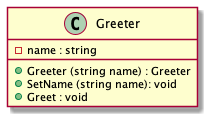
\includegraphics[width=0.35\textwidth]{../out/Documents/plantuml/encapsulation/encapsulation.png}
    \caption{The \texttt{Greeter} class}
    \label{uml.classes.greeter}
\end{wrapfigure}

Imagine a \textit{greeter} class, where a field contains the name of the person to greet. Here, the designers of the class might want to have stricter control of what clients are allowed to set this field to. It might make sense to disallow it to be set to an empty string or \texttt{null}.

Then, the designers would implement a setter method to set the field with appropriate error handling and to finish it a method that invokes the greeting.

\subsubsection*{Inheritance}

Inheritance is the concept of having classes that inherits behavior from parent classes. The parent classes are called \textit{super classes} and the child classes are called \textit{sub classes}. When considering a full inheritance hierarchy, we call moving up the hierarchy for \textit{generalizing} and moving down the hierarchy \textit{specializing}.

\begin{wrapfigure}{r}{0.4\textwidth}
    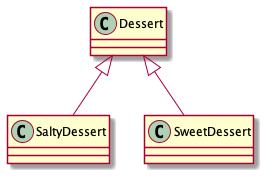
\includegraphics[width=0.35\textwidth]{../out/Documents/plantuml/inheritance/inheritance.png}
    \caption{The class hierarchy for desserts}
    \label{uml.classes.desserts}
\end{wrapfigure}

For example, we can imagine different kinds of desserts. We can naïvely divide them into salty desserts and sweet desserts. Here we define more specialized cases of desserts. We can thus say that \textit{"All salty desserts are desserts, but not all desserts are salty desserts"}.

\subsubsection*{Polymorphism}

Polymorphism is the concept of applying the same operations on different data types. 

Polymorphism can come on several flavors, but commonly it is used where different classes implement the same interface, and they are used in a place where the interface is used amongst a collection of possibly different types.


\begin{wrapfigure}{r}{0.4\textwidth}
    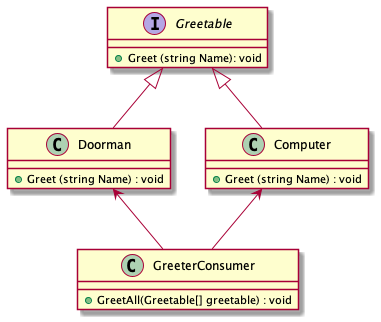
\includegraphics[width=0.4\textwidth]{../out/Documents/plantuml/polymorphism/polymorphism.png}
    \caption{Polymorphism in action with a commonly implemented interface}
    \label{uml.polymorphism}
\end{wrapfigure}

Polymorphism is also used with generic types, where we can make data structures such as lists, that are able to work with any type, because it manages the concrete instances of the types, but doesn't really depend on what the data types "can do".

I've attempted to illustrate this in the image to the right. Here we see an interface defined to contain the method \texttt{Greet}. Anyone who implements this interface will promise to be able to make a greeting. This can be classes of disjoint inheritance hierarchies.

The \texttt{GreeterConsumer} is a third party entity that is able to consume these \texttt{Greetable} entities and invoke their independently implemented \textit{Greet} methods.

\pagebreak
\section*{C\# Entities and their relationships}

The relationship shown in figure \ref{uml.relationships.user-task-tag} shows the multiplicity between \texttt{User}s, \texttt{Task}s and \texttt{Tag}s.

\begin{figure}[h]
    \center
    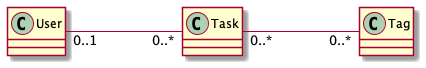
\includegraphics[width=0.6\textwidth]{../out/Documents/plantuml/exercise2/exercise2.png}
    \caption{The relationship between Users, Tasks and Tags with a focus on their multiplicity}
    \label{uml.relationships.user-task-tag}
\end{figure}

\section*{Task lifecycle and their State}

The following state diagram shows how a given Task's State will change over time in response to different operations.

\begin{figure}[h]
    \center
    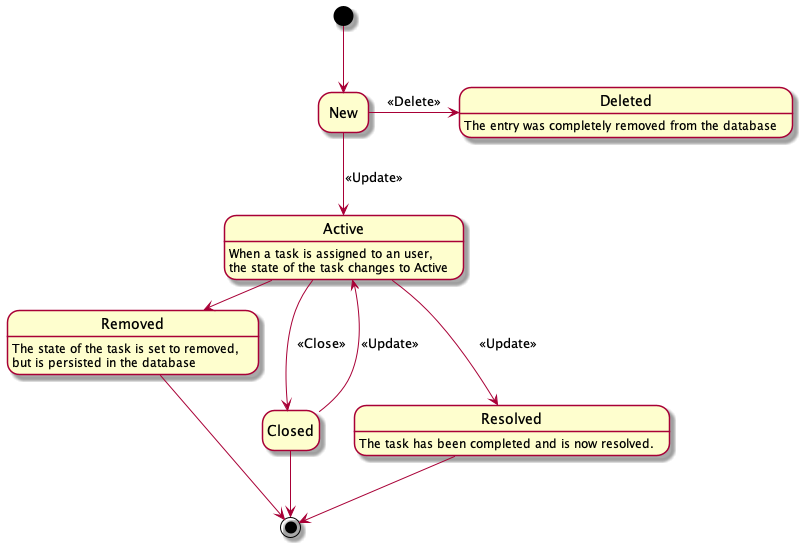
\includegraphics[scale=0.5]{../out/Documents/plantuml/exercise3/exercise3.png}
    \caption{The lifecycle of a Task and its State}
    \label{uml.exercise3}
\end{figure}

\pagebreak
\section*{Examples of violations of the SOLID principles}

\subsection*{Single Responsibility principle}

Violating the single responsibility principle means that classes will hold more than one responsibility in terms of what they are used for. This is illustrated below:

\begin{figure}[h]
    \centering
    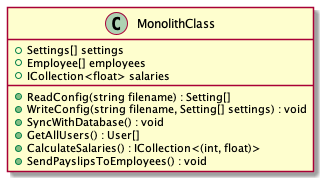
\includegraphics[scale=0.65]{../out/Documents/plantuml/exercise4_single_responsibility/exercise4_single_responsibility.png}
    \caption{Violation of the Single Responsibility principle.}
\end{figure}

\subsection*{Open/closed principle}

In object oriented programming, the principle about being allowed to extend existing functionality, but being prevented to modify it can be shown with a simple inheritance hierarchy.

To violate this principle, the designers of the general \texttt{Animal} class have not paid attention to sue of inappropriate access modifiers, such that sub classes of \texttt{Animal} can modify the previously defined methods and fields coming from the super class.

\begin{figure}[h]
    \centering
    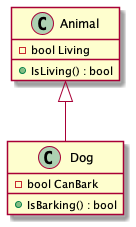
\includegraphics[scale=0.65]{../out/Documents/plantuml/exercise4_open_closed/exercise4_open_closed.png}
    \caption{}
\end{figure}

\subsection*{Liskov's substitution principle}

The following source code illustrates the missing use of Liskovs' substitution principle, where two classes of disjoint inheritance hierarchies implement the same function.

\begin{lstlisting}[language=Java]
class Dog
{
    public void Report()
    {
        Console.WriteLine("I'm a dog!");
    }
}

class Cat
{
    public void Report()
    {
        Console.WriteLine("I'm a cat!);
    }
}

class AnimalFactory
{
    public void reportAnimal(Object animal)
    {
        if (animal is Dog)
        {
            Dog dog = (Dog) animal;
            dog.Report();
        } else if (animal is Cat)
        {
            Cat cat = (Cat) animal;
            cat.Report();
        } else {
            Console.WriteLine("What animal even is this??");
        }
    }
}
\end{lstlisting}

\pagebreak
\subsection*{Interface segregation principle}

Here is an interface with too many different responsibilies, all that ultimately will serve a client, but they are of different responsibilies.

\begin{lstlisting}[language=Java]
interface IClientServable
{
  Report GetReport(int id);
  Report[] AllReports();
  int64 CalculateMonthlyPaycheckSum();
  int64 CalculateMonthlyCostsForHousing();
  Employee GetEmployee(int id);
  Employee[] AllEmployees();
  void SetDbContext(DBContext context);
  void SetLogger(Logger logger);
}
  
\end{lstlisting}

\subsection*{Dependency Inversion principle}

Here is a break on the Dependency Inversion principle, where another class, the \texttt{Logger} class is being composed by the \texttt{Worker} class to enable use of logging.

\begin{figure}[h]
  \centering
  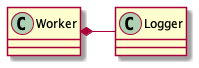
\includegraphics{../out/Documents/plantuml/exercise4_dependency_inversion/exercise4_dependency_inversion.png}
  \caption{The worker uses the Logger class throughout its lifecycle}
\end{figure}

\pagebreak
\section*{Solutions to the examples of broken SOLID principles}

\subsection*{Single Responsibility principle}

We split the monolith class into different classes based upon which methods share the same context of kind of responsibility.

\begin{figure}[h]
  \centering
  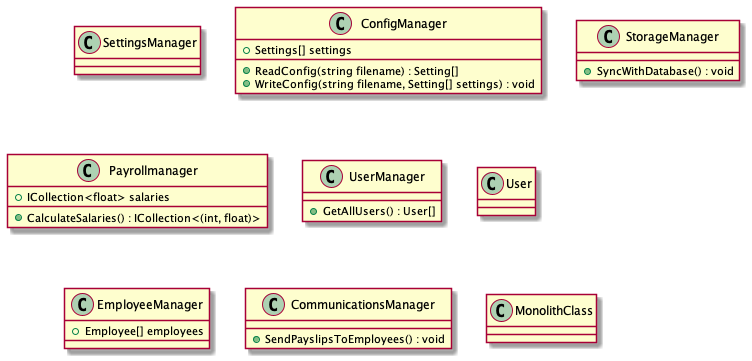
\includegraphics[scale=0.5]{../out/Documents/plantuml/exercise5_single_responsibility/exercise5_single_responsibility.png}
\end{figure}

\subsection*{Open/closed principle}

We disallow the Dog sub class to be able to override the \texttt{IsLiving()} method and \texttt{Living : bool} field from the Animal super class.

\begin{figure}[h]
  \centering
  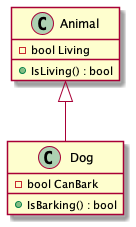
\includegraphics[scale=0.65]{../out/Documents/plantuml/exercise5_open_closed/exercise5_open_closed.png}
\end{figure}

\pagebreak
\subsection*{Liskov's substitution principle}

We fix the violation of the principle by using inheritance:

\begin{lstlisting}[language=Java]

  abstract class Animal
  {
    public virtual void Report();
  }

  class Dog : Animal
  {
      public void Report()
      {
          Console.WriteLine("I'm a dog!");
      }
  }
  
  class Cat : Animal
  {
      public void Report()
      {
          Console.WriteLine("I'm a cat!);
      }
  }
  
  class AnimalFactory
  {
      public void reportAnimal(Animal animal)
      {
          Animal.Report();
      }
  }
  \end{lstlisting}


\pagebreak
\subsection*{Interface segregation principle}

We fix the violation of the interface segregation principle by separating the giant monolithic interface smaller interfaces with higher cohesion:

\begin{lstlisting}[language=Java]
  interface IReportable
  {
    Report GetReport(int id);
    Report[] AllReports();
  }

  interface ICalculateable
  {
    int64 CalculateMonthlyPaycheckSum();
    int64 CalculateMonthlyCostsForHousing();
  }

  interface IEmployeeQueryable
  {
    Employee GetEmployee(int id);
    Employee[] AllEmployees();
  }

  interface IDbConfigurable
  {
    void SetDbContext(DBContext context);
  }

  interface ILoggerConfigurable
  {
    void SetLogger(Logger logger);
  }
\end{lstlisting}

\pagebreak
\subsection*{Dependency Inversion principle}

We employ constructer dependency injection to dynamically set the logger to use that implements the \texttt{ILoggerable} interface.

\begin{figure}[h]
  \centering
  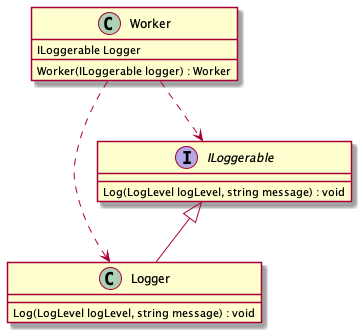
\includegraphics[scale=0.65]{../out/Documents/plantuml/exercise5_dependency_inversion/exercise5_dependency_inversion.png}
\end{figure}


\end{document}

